\section{Why Order Is Not Similarity}
\label{sec-order}

A sorted index answers a bound prefix with one range scan, and it is tempting
to hope that terms close in meaning are close in the order.
This section shows that no order can make them so, measures how far real
orders get, and so explains why \sys adds vector indexes instead of reordering
its trees.

\stitle{The order of the trees}.
A triple is a key of three dictionary ids compared with \texttt{memcmp}.
The dictionary assigns ids densely in first-seen order, and the loader interns
the terms of each statement in file order, so the order of every tree is the
order in which terms first appeared in the input.
Two classes are adjacent in the index only if they were adjacent in the file.

\begin{lemma}[Bandwidth]\label{lem-bw}
Let $G$ be a graph with $N$ vertices and diameter $D$.
In every linear order of the vertices some edge joins vertices at least
$(N-1)/D$ positions apart.
\end{lemma}
\begin{proof}
The first and last vertices of the order are $N-1$ apart and joined by a path
of at most $D$ edges, so some edge of the path covers at least $(N-1)/D$
positions.
\end{proof}

For the neighbor graph of a $d$-dimensional grid with $N=g^d$ points
(diameter $d(g-1)$), Lemma~\ref{lem-bw} gives $(g^d-1)/(d(g-1)) \ge g^{d-1}/d$
positions in any order, so a scan of width $w$ cannot contain all neighbors
unless $w$ is that large.
Space-filling curves keep neighbors close on average and need several scans to
cover a query ball; they do not escape the lemma.

\stitle{How much locality do real orders give?}
We took the Gene Ontology (release 2026-07-26 without obsolete terms: 38,092
classes and 57,456 \texttt{is\_a} edges), embedded each term's name with
\texttt{all-MiniLM-L6-v2}~\cite{reimers2019} ($d=384$), and for 2,000 random
terms took the ten nearest by cosine.
For each order of the terms, Table~\ref{tab-order} gives the share of those
neighbors within $\pm W$ positions.

\begin{table}[t]
\caption{Share of the 10 nearest neighbors (by cosine) found within $\pm W$ positions of a term, and the median position gap to the nearest neighbor. GO, 38,092 terms, 2,000 queries.}
\label{tab-order}
\small
\resizebox{\columnwidth}{!}{%
\begin{tabular}{@{}lrrrrrr@{}}
\toprule
Order & gap & $\pm$50 & $\pm$100 & $\pm$500 & $\pm$1000 & $\pm$5000 \\
\midrule
dictionary id (first seen) & 1739 & .195 & .211 & .258 & .284 & .438 \\
hierarchy, deepest parent & 45 & .328 & .377 & .498 & .561 & .735 \\
hierarchy, first parent & 37 & .319 & .366 & .481 & .546 & .726 \\
label, alphabetical & 1749 & .310 & .334 & .379 & .408 & .558 \\
random & 10823 & .003 & .005 & .024 & .049 & .242 \\
\bottomrule
\end{tabular}}
\end{table}

\begin{figure}[t]
\centering
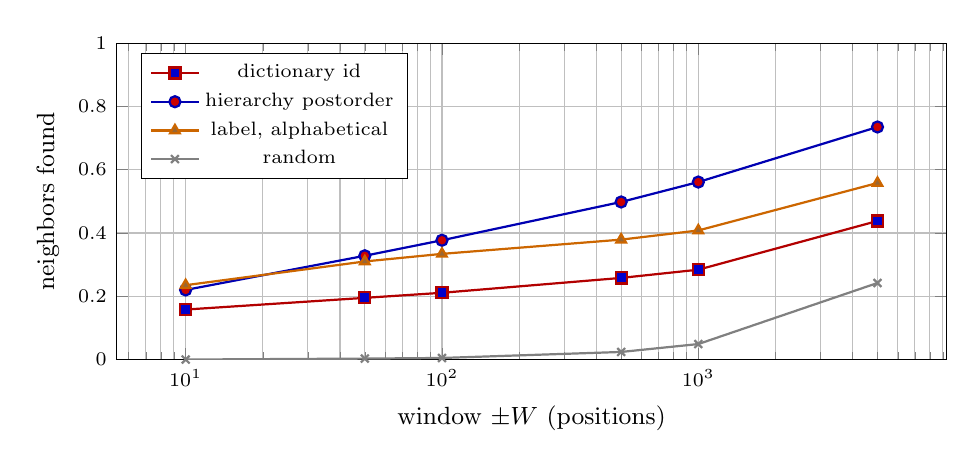
\begin{tikzpicture}
\begin{axis}[width=\columnwidth,height=5.6cm,xmode=log,xlabel={window $\pm W$ (positions)},ylabel={neighbors found},ymin=0,ymax=1,grid=both,legend pos=north west,legend style={font=\scriptsize},tick label style={font=\scriptsize},label style={font=\small}]
\addplot+[mark=square*,color=red!70!black,thick] coordinates {(10,0.158) (50,0.195) (100,0.211) (500,0.258) (1000,0.284) (5000,0.438)};
\addlegendentry{dictionary id}
\addplot+[mark=*,color=blue!70!black,thick] coordinates {(10,0.22) (50,0.328) (100,0.377) (500,0.498) (1000,0.561) (5000,0.735)};
\addlegendentry{hierarchy postorder}
\addplot+[mark=triangle*,color=orange!80!black,thick] coordinates {(10,0.235) (50,0.31) (100,0.334) (500,0.379) (1000,0.408) (5000,0.558)};
\addlegendentry{label, alphabetical}
\addplot+[mark=x,color=gray,thick] coordinates {(10,0) (50,0.003) (100,0.005) (500,0.024) (1000,0.049) (5000,0.242)};
\addlegendentry{random}
\end{axis}
\end{tikzpicture}

\caption{The data of Table~\ref{tab-order}: the share of neighbors found within $\pm W$ positions, by order.}
\label{fig-order}
\end{figure}

Three things follow.
First, the postorder of the class hierarchy is the best order, and much better
than first-seen ids: the nearest neighbor is 45 positions away instead of
1,739.
Second, even so, a scan of 100 positions finds 38\% of the ten neighbors, and
a window of $\pm$1,000 positions (2.6\% of the ontology) still misses 44\%;
Lemma~\ref{lem-bw} is not an artifact of the grid.
Third, first-seen ids are not random: the ontology's ids were minted in related
batches, so ids carry some locality (0.21 at $\pm$100) that depends on the file
and not on the engine.
Of the ten neighbors, 12\% are a parent or child and 32\% are within two
\texttt{is\_a} steps, while a two-step neighborhood holds only 45 terms
(0.12\% of the ontology), so hierarchy proximity is highly informative about
meaning without being sufficient.
The order is therefore useful for structure and not a substitute for a vector
index.
